\chapter{Architettura software}
\label{cap:architetturasw}

Per semplificare l'implementazione e agevolare il riuso del codice esistente, il software è stato realizzato utilizzando ROS (Robot Operating System) \cite{rosweb}. Si tratta di un middleware appositamente sviluppato per applicazioni robotiche, costituite da un elevato numero di moduli relativamente indipendenti che interagiscono tra loro.

Un sistema realizzato con ROS è suddiviso in un certo numero di \emph{nodi}, ovvero semplici processi\footnote{attualmente ROS supporta C++ e Python} indipendenti ed eseguiti in parallelo, che svolgono ciascuno una funzione elementare. Per migliorare l'organizzazione e la distribuzione dei sorgenti, i nodi possono poi essere raggruppati in \emph{package}. A loro volta, un gruppo di package può formare uno \emph{stack}.

ROS mette a disposizione due differenti tecniche con cui i nodi possono comunicare tra loro:
\begin{itemize}
 \item un paradigma ``publish-subscribe'': i nodi inviano (pubblicano) \emph{messaggi} su un certo \emph{argomento} (\emph{topic}), che vengono ricevuti dai nodi iscritti (subscribe), destinatari della comunicazione
 \item l'invocazione di \emph{servizi} esposti da altri nodi, secondo una semantica simile a quella di una chiamata a funzione
\end{itemize}

Oltre a funzionare come middleware di comunicazione interprocesso, ROS mette a disposizione alcuni programmi e librerie aggiuntive che svolgono funzioni utili allo sviluppo di applicazioni robotiche.

Il sistema realizzato risulta composto da vari nodi, ciascuno contenuto in un omonimo package all'interno della directory principale del progetto. I nodi, dettagliati nei paragrafi successivi, sono rappresentati nella figura \ref{fig:schemanodi}, insieme alle loro interfacce (messaggi scambiati e servizi esposti) e alle principali interazioni con le altre librerie utilizzate (esterne a ROS) e/o l'hardware.

\begin{figure}[h]
\resizebox{\linewidth}{!}{%
\begin{tikzpicture}[node distance=1cm, auto]
\tikzset{
   mynode/.style={rectangle,rounded corners,draw=black, top color=white, bottom color=white!50, thick, inner sep=1em, minimum size=3em, text centered},
   mynode2/.style={rectangle,rounded corners,draw=black, top color=white, bottom color=white!50, dashed, inner sep=1em, minimum size=1em, text centered},
}  
\node[mynode] (spykee) {\textbf{SpyKee}}; 
\node[mynode, below=4cm of spykee] (echoes) {\textbf{Echoes}}; 
\node[mynode, right=5cm of spykee] (vision) {\textbf{Vision}}; 
\node[mynode, below right=3cm of vision] (isaac) {\textbf{IsAac}}; 
\node[mynode2, below=1cm of isaac] (brian) {\emph{Mr. BRIAN}}; 
\node[mynode2, below left= 2cm of spykee] (robot) {\emph{Robot}}; 
\node[mynode2, above=1cm of vision] (opencv) {\emph{OpenCV + Blob Growing Algorithm}}; 
 
\draw[->, >=latex', shorten >=2pt, shorten <=2pt, bend left=10, thick] 
     (spykee.east) to node[auto, swap] {\ttfamily{spykee\_camera}}(vision.west); 

\draw[->, >=latex', shorten >=2pt, shorten <=2pt, bend left=10, thick] 
     (isaac.west) to node[auto, swap] {\ttfamily{spykee\_motion}}(spykee.south); 

\draw[->, >=latex', shorten >=2pt, shorten <=2pt, bend right=20, thick] 
     (echoes.east) to node[auto,swap] {\ttfamily{\begin{tabular}{c}
	 sonar\_data \\
     rfid\_data \\
     towers\_data
  \end{tabular}
}}(isaac.west); 
     
\draw[->, >=latex', shorten >=2pt, shorten <=2pt, bend right=10, thick, dashed] 
     (isaac.west) to node[auto, swap] {{\ttfamily{led\_data}} (servizio)}(echoes.east); 

\draw[->, >=latex', shorten >=2pt, shorten <=2pt, bend left=30, thick] 
     (vision.east) to node[auto, swap] {{\ttfamily{vision\_results}}}(isaac.north); 

\draw[<->, >=latex', shorten >=2pt, shorten <=2pt, bend left=0, thin, dashed] 
     (isaac.south) to node[auto, swap] {}(brian.north); 

\draw[<->, >=latex', shorten >=2pt, shorten <=2pt, bend left=0, thin, dashed] 
     (vision.north) to node[auto, swap] {}(opencv.south); 

\draw[<->, >=latex', shorten >=2pt, shorten <=2pt, bend left=7, thin, dashed] 
     (robot.north) to node[auto, swap] {Wi-fi}(spykee.west); 

\draw[<->, >=latex', shorten >=2pt, shorten <=2pt, bend right=7, thin, dashed] 
     (robot.south) to node[auto, swap] {Zigbee}(echoes.west); 

% The swap command corrects the placement of the text.

\end{tikzpicture} 
} 
\medskip

\caption{Struttura generale del sistema} 
\label{fig:schemanodi}
\end{figure}

\section{SpyKee}
Il nodo \emph{SpyKee} si occupa di interfacciare l'unità di elaborazione con le funzioni del robot che comunicano via Wi-Fi: permette di fornire i comandi ai cingoli e di ricevere le immagini catturate dalla telecamera. Questo nodo è frutto dell'adattamento a ROS di una libreria realizzata nei precedenti progetti analizzando mediante tramite un software di cattura dei pacchetti di rete la comunicazione tra il robot e il software di controllo fornito dalla Meccano.

SpyKee pubblica messaggi di tipo \verb|std_msgs::CompressedImage| sull'argomento \verb|spykee_camera|, che contengono le immagini ricevute dalla telecamera compresse in formato JPEG. Inoltre il nodo sottoscrive messaggi di tipo \verb|SpyKee::Motion| sull'argomento \verb|spykee_motion|, contenenti i comandi da inviare ai cingoli. Tali comandi sono costituiti da due interi compresi tra $-90$ e $90$, che rappresentano la velocità tangenziale e angolare del robot, e vengono convertiti dal nodo nei corrispondenti comandi al cingolo destro e sinistro.

\section{Echoes}
Il nodo \emph{Echoes} comunica via Zigbee con l'hardware aggiunto a posteriori al robot: sonar, led, lettore RFID, e ricevitori dei comandi inviati dagli interruttori posti sulle torri e sulle fabbriche.

Il nodo riceve i dati dalla porta seriale\footnote{di default viene utilizzato il device \texttt{/dev/ttyUSB0}, altrimenti il percorso del dispositivo deve essere fornito da riga di comando come primo argomento}, effettua il parsing delle stringhe ricevute, e pubblica i messaggi contenenti i dati rilevati:
\begin{itemize}
	\item \verb|Echoes::Sonar|, sull'argomento \verb|sonar_data|, contenenti i dati ricevuti dai sonar (valori delle distanze dei quattro sonar montati sul robot, espresse in millimetri).
	\item \verb|Echoes::Rfid|, sull'argomento \verb|rfid_data|, contenenti semplicemente una stringa identificativa del tag RFID rilevato
	\item \verb|Echoes::Tower| sull'argomento \verb|towers_data|, contenente un intero che corrisponde all'id della torre (o della fabbrica) abbattuta
\end{itemize}
Inoltre, il nodo espone un servizio di tipo \verb|Echoes::Led| che permette di controllare l'accensione dei led, e un altro servizio che consente di spegnere tutti i led. I led possono essere impostati nello stato di acceso, spento o lampeggiante. In particolare, per i led gialli e i led rossi, lo stato lampeggiante viene definito a livello dell'intero gruppo di led.

A causa dell'alto rumore presente nei valori provenienti dai sonar, il valore che viene pubblicato sul topic \verb|sonar_data| è filtrato attraverso un filtro a media mobile esponenziale. Questo significa che il dato pubblicato all'arrivo del $k$-esimo campione $x_{cur}$ registrato dal sonar è dato da %TODO sicuri che alpha = 0.3?!?
  \[ x_k = \alpha x_{cur} + (1 - \alpha) x_{k-1} \]
dove $\alpha = 0.3$, valore sufficientemente alto da rendere l'aggiornamento dei sonar abbastanza veloce per poter evitare efficacemente l'ostacolo, e sufficientemente basso da ridurre il rumore ad alta frequenza presente nel segnale.

\section{Vision: identificazione degli oggetti}

\emph{Vision} si occupa di analizzare le immagini provenienti dalla telecamera di Spykee, per rilevare la presenza di una torre o di una fabbrica. 

Riceve da \emph{SpyKee} i messaggi contenenti le immagini e, analizzata l'immagine, pubblica un messaggio di tipo \verb|Vision::Results| sull'argomento \verb|vision_results|. Questo messaggio contiene contenente i dati riguardanti gli oggetti trovati: in particolare, la posizione rispetto al centro dell'immagine, una stima della distanza in centimetri, e l'altezza e la larghezza del blob in pixel.

Il cuore del nodo è un algoritmo, già utilizzato nel progetto \cite{docmandelli}, che si occupa di identificare all'interno dell'immagine dei blob sufficientemente uniformi e di colore ``simile'' a quello degli oggetti che si stanno cercando. L'analisi viene effettuata basandosi su un algoritmo di tipo KNN, che necessita di una prima fase di addestramento. Al termine di questa fase, viene generato un classificatore (contenuto in un file \verb|.kcc|), tramite il quale l'algoritmo è in grado di associare ad ogni pixel dell'immagine una classe di identificazione. Le classi definite riguardano i pixel di colore simile a quello di una ``torre'' (classe R), oppure di una ``fabbrica'' (classe G). Una volta effettuata la classificazione dei pixel dell'immagine, viene eseguito un algoritmo per rilevare all'interno dell'immagine i blob di interesse, e quindi stabilire se all'interno dell'immagine è presente una torre o una fabbrica.

Il classificatore viene generato a partire da un file che contiene semplicemente un elenco di valori \verb|BGR| di pixel che si considerano del colore cercato. Per generare questo file è possibile utilizzare il nodo \emph{LittleEndian}: questo nodo carica le immagini da file oppure le riceve direttamente da \emph{SpyKee}, e consente di evidenziare nell'immagine le aree che corrispondono agli oggetti cercati, generando un file \verb|.dts| contenente l'insieme dei valori. A questo punto, per generare il classificatore, è sufficiente lanciare la prima volta \emph{Vision} indicando come parametro \verb|-L <filename.dts>|.

%TODO filtraggio etc?

\begin{nota}
È necessario prestare particolare attenzione nel training del classificatore, in quanto è una fase critica per il corretto funzionamento del gioco e il corretto riconoscimento degli oggetti. %% TODO TODO STA ROBA E' DA SISTEMARE!!!
\end{nota}

\section{RoboTower\_Game: la logica di gioco}
\begin{figure}
\centering
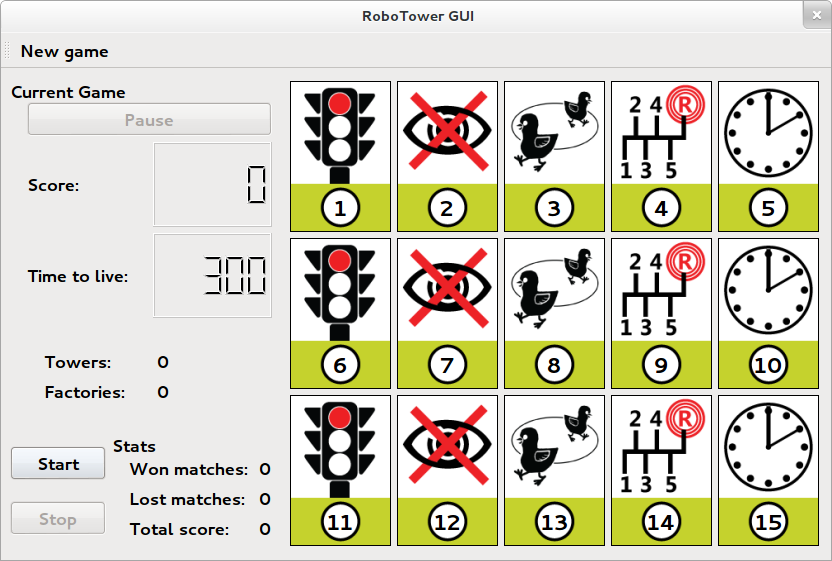
\includegraphics[scale=0.4]{images/rtgame}
\caption{Schermata principale dell'interfaccia di controllo del gioco}
\end{figure}

\emph{RoboTower\_Game} gestisce la logica ad ``alto livello'' del gioco e la comunicazione con l'utente tramite un'apposita interfaccia grafica, realizzata con le librerie Qt \cite{qtweb}. Si occupa di avviare e arrestare le partite, gestire lo stato del gioco, contare i punti, e tenere alcune semplici statistiche. Il nodo interagisce con gli altri processi:

\begin{itemize}
\item avviando e fermando il comportamento di basso livello del robot, a seconda dello stato corrente del gioco (mediante messaggi sull'argomento \verb|isaac_enable|)
\item ricevendo da \verb|Echoes| gli ID dei tag RFID letti e le informazioni riguardanti eventuali abbattimenti di torri o fabbriche
\item pubblicando messaggi relativi alle azioni speciali che devono essere eseguite, come spiegato nel seguito (argomento \verb|rfid_actions|), e invocando i servizi relativi all'accensione e allo spegnimento dei led relativi al punteggio
\end{itemize}

La maggior parte delle impostazioni di RoboTower\_Game possono essere configurate modificando sul file \verb|robotower.xml|, che si trova nella directory \verb|RoboTower_Game|. Un esempio di file di configurazione corretto è riportato in figura \ref{fig:configfile}\footnote{per semplicità sono stati omessi alcuni tag RFID e le relative azioni}. Il file di configurazione permette di specificare:
\begin{itemize}
\item I tempi del gioco (tag \lstinline|<time>|): la durata massima di un round del gioco (\lstinline|timetolive|), il tempo trascorso dall'inizio della partita (pressione del pulsante ``start'') e l'inizio del movimento del robot (\lstinline|setuptime|)
\item I parametri con cui viene calcolato il punteggio (tag \lstinline|<points>|): durante la partita, ogni secondo viene aggiunto un certo numero di punti per ogni torre e fabbrica che non sono stati ancora distrutti, definiti dagli attributi \lstinline|tower| e \lstinline|factory|
\item I parametri relativi a torre e fabbriche (tag \lstinline|<goals>|): in particolare, il numero di fabbriche (\lstinline|factories|) e l'id dell'obiettivo che dev'essere considerato come torre (\lstinline|towerid|)
\end{itemize}

\begin{figure}
{
\lstset{
  language=XML,
  morekeywords={encoding, robotower, config, time, points, goal, rfid, action, tag}}
\begin{lstlisting}
<robotower>
   <config>
      <time timetolive="300" setuptime="30" />
      <points tower="100" factory="30" />
      <goals towerid="4" factories="3" />
   </config>

   <rfid>
      <action name="lock_all">
         <tag id="4400F56CD1" num="1" />
         <tag id="4400F59195" num="2" />
         <tag id="4400F58B6D" num="3" />
      </action>
      
      <action name="disable_vision">
         <tag id="4400BDB1D9" num="4" />
         <tag id="4400BDC253" num="5" />
         <tag id="4B00DA3279" num="6" />
      </action>
   </rfid>
</robotower>
\end{lstlisting}
}
\caption{Il file di configurazione}
\label{fig:configfile}
\end{figure}

Il nodo si occupa inoltre di gestire i comportamenti ``speciali'' (action) del robot, attivati quando il robot si avvicina ai tag RFID cui sono associate. Per ogni trappola, è necessario specificare all'interno del blocco \lstinline|<action>| relativo all'azione associata, l'id e un numero (univoco) utilizzato per identificarlo nell'interfaccia grafica. Le azioni che possono essere specificate (parametri \lstinline|name|) sono:
\begin{itemize}
\item \lstinline|lock_all| blocca per 5 secondi i motori del robot
\item \lstinline|force_rotate| costringe per 5 secondi il robot a ruotare su se stesso, inibendo i comandi diretti a uno dei due cingoli
\item \lstinline|disable_vision| disabilita la visione del robot per 5 secondi
\item \lstinline|go_back| blocca per 5 secondi l'avanzamento del robot, costringendolo a tornare indietro
\item \lstinline|modify_time| modifica casualmente il tempo rimanente alla fine del round (sia in positivo che in negativo)
\end{itemize}
Una volta che viene letto un tag, questo viene disabilitato. I tag possono essere ricaricati, uno alla volta, dopo un periodo di tempo che dipende dal numero di fabbriche residue sul campo di gioco. %TODO RENDERLO CONFIGURABILE

\section{IsAac: il comportamento del robot}
\emph{IsAac} si occupa di controllare il comportamento di ``basso livello'' del robot durante il gioco. In base ai dati provenienti dai sensori, gestisce il comportamento del robot (i set-point per i cingoli e l'accensione di alcuni led).

Il nodo riceve i messaggi pubblicati da \emph{Echoes} e \emph{Vision}, e invia comandi a \emph{SpyKee} (messaggi \verb|Spykee::Motion| sull'argomento \verb|spykee_motion|) riguardanti il controllo dei cingoli. Inoltre invoca il servizio \verb|led_data| esposto da Echoes per il controllo dei led gialli e del led verde posti sul robot. I led gialli lampeggiano quando \emph{IsAac} è attivo, sono spenti quando non è attivo, e sono accesi fissi quando il robot è bloccato in una trappola. Il led verde lampeggia quando viene rilevata una torre o una fabbrica, altrimenti è spento.

Il nodo riceve da \emph{RoboTower\_Game} i comandi di attivazione e disattivazione, e le informazioni riguardanti il blocco del robot in una trappola associata ad un'azione che prevede la modifica dei comandi provenienti dai sensori oppure diretti agli attuatori (le altre azioni sono implementate direttamente in \emph{RoboTower\_Game}.

Per l'implementazione di questo nodo, è stata sfruttata la libreria Mr. Brian, sviluppata dal Politecnico di Milano all'interno di MRT \cite{mrt}. Questa libreria consente di definire il comportamento da applicare al robot come un insieme di regole scritte in logica fuzzy, utilizzando anche predicati che risultano dalla fuzzyficazione degli ingressi. La configurazione di Brian è basata su un insieme di file di testo: in questo modo è possibile modificare totalmente i comportamenti senza bisogno di ricompilare il codice sorgente. I file di configurazione, presenti nella cartella \verb|IsAac/config|, sono:
\begin{itemize}
\item \verb|behaviour.txt| contiene l'elenco, suddiviso per livelli, dei comportamenti (regole) definiti, ognuno dei quali è contenuto in un file \verb|.rul|
\item \verb|ctof.txt| associa ad ogni dato in ingresso (crisp) una membership function, che verrà utilizzata per la fase di fuzzyficazione. Le membership function sono definite nel file \verb|shape_ctof.txt|.
\item \verb|s_ftoc.txt| Definisce i valori in uscita e li associa alle funzioni definite nel file \verb|s_shape.txt|
\item \verb|Predicate.ini| Definisce i predicati fuzzy sulla base delle variabili fuzzy e/o di altri predicati
\item \verb|Cando.ini| Definisce le condizioni di attivazione per un determinato comportamento (le condizioni necessarie per cui eseguire quel comportamento sia sensato)
\item \verb|want.txt| Definisce le condizioni per cui è opportuno attivare un determinato comportamento
\end{itemize}
All'interno del manuale di MRT \cite{mrtmanual} è presente la descrizione completa del funzionamento di Mr. Brian e della sintassi dei file di configurazione.

I comportamenti che sono stati implementati riguardano:
\begin{itemize}
 \item Cercare casualmente la torre o le fabbriche (Search.rul)
 \item Raggiungere la torre o la fabbrica, una volta che è stata trovata (GoToTower.rul e GoToFactory.rul)
 \item Evitare gli ostacoli (AvoidObstacle.rul, KeepDistance.rul, GoBack.rul)
 \item Distruggere la torre o una fabbrica (Destroy.rul)
\end{itemize}

%TODO dettagliare meglio le regole o il loro funzionamento, spiegare la suddivisione in livelli???